\documentclass[11pt]{article}

    \usepackage{tocloft}

    \cftsetindents{section}{0em}{2em}
    \cftsetindents{subsection}{0em}{2em}

    \renewcommand\cfttoctitlefont{\hfill\Large\bfseries}
    \renewcommand\cftaftertoctitle{\hfill\mbox{}}
    \setcounter{tocdepth}{2}
    \usepackage{listings}
    \usepackage{color}
    \usepackage{url}
    \definecolor{codegreen}{rgb}{0,0.6,0}
    \definecolor{codegray}{rgb}{0.5,0.5,0.5}
    \definecolor{codepurple}{rgb}{0.58,0,0.82}
    \definecolor{backcolour}{rgb}{0.95,0.95,0.92}
    \usepackage{algpseudocode} 
    \usepackage{algorithm} 
    \lstdefinestyle{mystyle}{
    backgroundcolor=\color{backcolour},   
    commentstyle=\color{codegreen},
    keywordstyle=\color{blue},
    stringstyle=\color{codepurple},
    basicstyle=\footnotesize,
    breakatwhitespace=false,         
    breaklines=true,                 
    captionpos=b,                    
    keepspaces=true,                 
    numbers=left,                    
    numbersep=5pt,                  
    showspaces=false,                
    showstringspaces=false,
    showtabs=false,                  
    tabsize=3
    }
    
    \lstset{ 
    style=mystyle,
    basicstyle=\small\ttfamily,
    breaklines=true
    }
    \usepackage{seqsplit}    
    \usepackage[T1]{fontenc}


    % Nicer default font than Computer Modern for most use cases
    \usepackage{palatino}

    % Basic figure setup, for now with no caption control since it's done
    % automatically by Pandoc (which extracts ![](path) syntax from Markdown).
    \usepackage{graphicx}
    % We will generate all images so they have a width \maxwidth. This means
    % that they will get their normal width if they fit onto the page, but
    % are scaled down if they would overflow the margins.
    \makeatletter
    \def\maxwidth{\ifdim\Gin@nat@width>\linewidth\linewidth
    \else\Gin@nat@width\fi}
    \makeatother
    \let\Oldincludegraphics\includegraphics
    % Set max figure width to be 80% of text width, for now hardcoded.
    \renewcommand{\includegraphics}[1]{\Oldincludegraphics[width=.8\maxwidth]{#1}}
    % Ensure that by default, figures have no caption (until we provide a
    % proper Figure object with a Caption API and a way to capture that
    % in the conversion process - todo).
    \usepackage{caption}
    \DeclareCaptionLabelFormat{nolabel}{}
    \captionsetup{labelformat=nolabel}

    \usepackage{adjustbox} % Used to constrain images to a maximum size 
    \usepackage{xcolor} % Allow colors to be defined
    \usepackage{enumerate} % Needed for markdown enumerations to work
    \usepackage{geometry} % Used to adjust the document margins
    \usepackage{amsmath} % Equations
    \usepackage{amssymb} % Equations
    \usepackage{textcomp} % defines textquotesingle
    % Hack from http://tex.stackexchange.com/a/47451/13684:
    \AtBeginDocument{%
        \def\PYZsq{\textquotesingle}% Upright quotes in Pygmentized code
    }
    \usepackage{upquote} % Upright quotes for verbatim code
    \usepackage{eurosym} % defines \euro
    \usepackage[mathletters]{ucs} % Extended unicode (utf-8) support
    \usepackage[utf8x]{inputenc} % Allow utf-8 characters in the tex document
    \usepackage{fancyvrb} % verbatim replacement that allows latex
    \usepackage{grffile} % extends the file name processing of package graphics 
                         % to support a larger range 
    % The hyperref package gives us a pdf with properly built
    % internal navigation ('pdf bookmarks' for the table of contents,
    % internal cross-reference links, web links for URLs, etc.)
\usepackage[pdftex,
            pdfauthor={BDSMasters: Efstratios Gounidellis, Lamprini Koutsokera},
            pdftitle={k-means algorithm implementation on Hadoop},
            pdfsubject={Big Data Management Systems},
            pdfkeywords={hadoop; mapreduce; kmeans; dmst; aueb; python; mrjob},
            pdfproducer={Latex with hyperref},
            pdfcreator={pdflatex}]{hyperref}
    \usepackage{longtable} % longtable support required by pandoc >1.10
    \usepackage{booktabs}  % table support for pandoc > 1.12.2
    \usepackage[normalem]{ulem} % ulem is needed to support strikethroughs (\sout)
                                % normalem makes italics be italics, not underlines
    

    
    
    % Colors for the hyperref package
    \definecolor{urlcolor}{rgb}{0,.145,.698}
    \definecolor{linkcolor}{rgb}{.71,0.21,0.01}
    \definecolor{citecolor}{rgb}{.12,.54,.11}

    % ANSI colors
    \definecolor{ansi-black}{HTML}{3E424D}
    \definecolor{ansi-black-intense}{HTML}{282C36}
    \definecolor{ansi-red}{HTML}{E75C58}
    \definecolor{ansi-red-intense}{HTML}{B22B31}
    \definecolor{ansi-green}{HTML}{00A250}
    \definecolor{ansi-green-intense}{HTML}{007427}
    \definecolor{ansi-yellow}{HTML}{DDB62B}
    \definecolor{ansi-yellow-intense}{HTML}{B27D12}
    \definecolor{ansi-blue}{HTML}{208FFB}
    \definecolor{ansi-blue-intense}{HTML}{0065CA}
    \definecolor{ansi-magenta}{HTML}{D160C4}
    \definecolor{ansi-magenta-intense}{HTML}{A03196}
    \definecolor{ansi-cyan}{HTML}{60C6C8}
    \definecolor{ansi-cyan-intense}{HTML}{258F8F}
    \definecolor{ansi-white}{HTML}{C5C1B4}
    \definecolor{ansi-white-intense}{HTML}{A1A6B2}

    % commands and environments needed by pandoc snippets
    % extracted from the output of `pandoc -s`
    \providecommand{\tightlist}{%
      \setlength{\itemsep}{0pt}\setlength{\parskip}{0pt}}
    \DefineVerbatimEnvironment{Highlighting}{Verbatim}{commandchars=\\\{\}}
    % Add ',fontsize=\small' for more characters per line
    \newenvironment{Shaded}{}{}
    \newcommand{\KeywordTok}[1]{\textcolor[rgb]{0.00,0.44,0.13}{\textbf{{#1}}}}
    \newcommand{\DataTypeTok}[1]{\textcolor[rgb]{0.56,0.13,0.00}{{#1}}}
    \newcommand{\DecValTok}[1]{\textcolor[rgb]{0.25,0.63,0.44}{{#1}}}
    \newcommand{\BaseNTok}[1]{\textcolor[rgb]{0.25,0.63,0.44}{{#1}}}
    \newcommand{\FloatTok}[1]{\textcolor[rgb]{0.25,0.63,0.44}{{#1}}}
    \newcommand{\CharTok}[1]{\textcolor[rgb]{0.25,0.44,0.63}{{#1}}}
    \newcommand{\StringTok}[1]{\textcolor[rgb]{0.25,0.44,0.63}{{#1}}}
    \newcommand{\CommentTok}[1]{\textcolor[rgb]{0.38,0.63,0.69}{\textit{{#1}}}}
    \newcommand{\OtherTok}[1]{\textcolor[rgb]{0.00,0.44,0.13}{{#1}}}
    \newcommand{\AlertTok}[1]{\textcolor[rgb]{1.00,0.00,0.00}{\textbf{{#1}}}}
    \newcommand{\FunctionTok}[1]{\textcolor[rgb]{0.02,0.16,0.49}{{#1}}}
    \newcommand{\RegionMarkerTok}[1]{{#1}}
    \newcommand{\ErrorTok}[1]{\textcolor[rgb]{1.00,0.00,0.00}{\textbf{{#1}}}}
    \newcommand{\NormalTok}[1]{{#1}}
    
    % Additional commands for more recent versions of Pandoc
    \newcommand{\ConstantTok}[1]{\textcolor[rgb]{0.53,0.00,0.00}{{#1}}}
    \newcommand{\SpecialCharTok}[1]{\textcolor[rgb]{0.25,0.44,0.63}{{#1}}}
    \newcommand{\VerbatimStringTok}[1]{\textcolor[rgb]{0.25,0.44,0.63}{{#1}}}
    \newcommand{\SpecialStringTok}[1]{\textcolor[rgb]{0.73,0.40,0.53}{{#1}}}
    \newcommand{\ImportTok}[1]{{#1}}
    \newcommand{\DocumentationTok}[1]{\textcolor[rgb]{0.73,0.13,0.13}{\textit{{#1}}}}
    \newcommand{\AnnotationTok}[1]{\textcolor[rgb]{0.38,0.63,0.69}{\textbf{\textit{{#1}}}}}
    \newcommand{\CommentVarTok}[1]{\textcolor[rgb]{0.38,0.63,0.69}{\textbf{\textit{{#1}}}}}
    \newcommand{\VariableTok}[1]{\textcolor[rgb]{0.10,0.09,0.49}{{#1}}}
    \newcommand{\ControlFlowTok}[1]{\textcolor[rgb]{0.00,0.44,0.13}{\textbf{{#1}}}}
    \newcommand{\OperatorTok}[1]{\textcolor[rgb]{0.40,0.40,0.40}{{#1}}}
    \newcommand{\BuiltInTok}[1]{{#1}}
    \newcommand{\ExtensionTok}[1]{{#1}}
    \newcommand{\PreprocessorTok}[1]{\textcolor[rgb]{0.74,0.48,0.00}{{#1}}}
    \newcommand{\AttributeTok}[1]{\textcolor[rgb]{0.49,0.56,0.16}{{#1}}}
    \newcommand{\InformationTok}[1]{\textcolor[rgb]{0.38,0.63,0.69}{\textbf{\textit{{#1}}}}}
    \newcommand{\WarningTok}[1]{\textcolor[rgb]{0.38,0.63,0.69}{\textbf{\textit{{#1}}}}}
    
    
    % Exact colors from NB
    \definecolor{incolor}{rgb}{0.0, 0.0, 0.5}
    \definecolor{outcolor}{rgb}{0.545, 0.0, 0.0}



    
    % Prevent overflowing lines due to hard-to-break entities
    \sloppy 
    % Setup hyperref package
    \hypersetup{
      breaklinks=true,  % so long urls are correctly broken across lines
      colorlinks=true,
      urlcolor=urlcolor,
      linkcolor=linkcolor,
      citecolor=citecolor,
      }
    % Slightly bigger margins than the latex defaults
    
    \geometry{verbose,tmargin=1in,bmargin=1in,lmargin=1in,rmargin=1in}
    
\newcommand{\horrule}[1]{\rule{\linewidth}{#1}} % command for creating lines to place the title in a box

\title{
    \horrule{0.5pt} \\ [0.4cm]
    \huge  k-means algorithm implementation on Hadoop\\
    \horrule{2pt} \\[0.5cm]	
\vspace{10px}
}

\author{\large Efstratios Gounidellis\\stratos.gounidellis [at] gmail.com \\ \\ \\ 
		Lamprini Koutsokera\\lkoutsokera [at] gmail.com \\ \\ \\ \\ \\ \\ \\ \\
Course: "Big Data Management Systems"
\\
Professor: Damianos Chatziantoniou
\\ \\ \\
\vspace{40px}
Department of Management Science \& Technology
\\ School of Business
\\
Athens University of Economics \& Business} % Author's name

\date{
\vfill \large\today} % Today's date    



    \begin{document}
    
\maketitle

\pagebreak 

\tableofcontents

\pagebreak 
    
\section{Data points generation}\label{data-points-generation}

\subsection{createDataPoints.py}\label{createdatapoints.py}

The initial task of the project is to generate a set of more than one
million data points to be used later as input for the k-means
clustering algorithm. Using this python script three isotropic Gaussian
blobs for clustering are generated. More specifically, the centers are
the following data points {[}25, 25{]}, {[}-1, -1{]}, {[}-25, -25{]}.
Additionally, the data points are presented visually with the use of a
scatter plot.
\begin{center}
	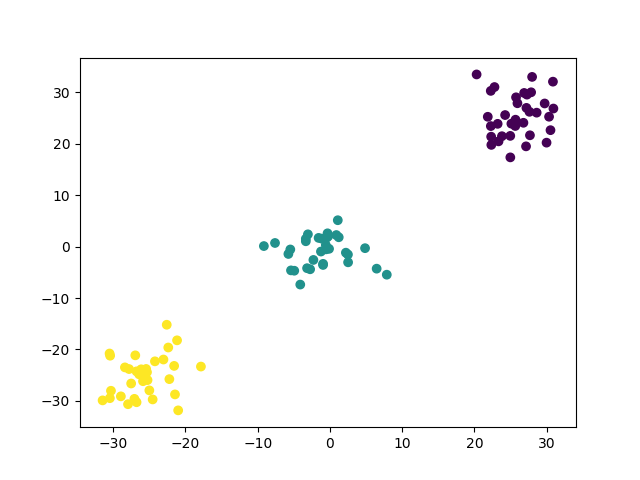
\includegraphics{../images/data_points.png}\\
\end{center}
\begin{lstlisting}  [language=Python]
"""createDataPoints.py: Generate data points for clustering."""

import argparse
import matplotlib.pyplot as plt
import os
import pandas as pd
from sklearn.datasets.samples_generator import make_blobs

__author__ = "Stratos Gounidellis, Lamprini Koutsokera"
__copyright__ = "Copyright 2017, BDSMasters"


class DataGenerator():

    def generateData(self, points, dataFile):
        """Generate the input data points.

        :param self: An instance of the class DataGenerator.
        :param points: The number of data points to be generated.
        :param dataFile: The file to save the data points.
        """
        centers = [[25, 25], [-1, -1], [-25, -25]]
        X, labels_true = make_blobs(n_samples=long(points),
                                    centers=centers, cluster_std=3.5,
                                    n_features=2)

        df = pd.DataFrame(X)
        df.to_csv(dataFile, header=False, index=False, sep=" ")

        plt.scatter(X[:, 0], X[:, 1], c=labels_true)
        directory = "../images"
        if not os.path.isdir(directory):
            os.makedirs(directory)
        plt.savefig("../images/data_points.png")


if __name__ == "__main__":
    parser = argparse
    parser = argparse.ArgumentParser()
    parser.add_argument("dataFile", type=str,
                        help="File to save the generated data points.")

    parser.add_argument("points", type=int,
                        help="Number of data points to create.")
    args = parser.parse_args()
    instanceDataGenerator = DataGenerator()
    instanceDataGenerator.generateData(args.points, args.dataFile)

\end{lstlisting}

    

\section{Number of clusters}\label{number-of-clusters}

\subsection{plotSilhouetteScore.py }\label{plotsilhouettescore.py}

The silhouette score constitutes a useful criterion for determining the proper number of clusters and it was firstly suggested by Peter J. Rousseeuw. The silhouette shows which objects lie well within their cluster, and which ones are merely somewhere in between clusters. A silhouette close to 1 implies the datum is in an appropriate cluster, while a silhouette close to −1 implies the datum is in the wrong cluster. \par 
The following python script calculates the silhouette score for different numbers of clusters ranging from 2 to 6. With this script not only the average silhouette score of each cluster is visualized but also the thickness (i.e.~the number of data points) of each cluster. The number of clusters which leads to clusters of more or less similar thickness and silhouette score above the average could be the optimal number of clusters for the k-means algorithm. \par
As expected creating three clusters is the optimal solution in this case.
\begin{center}
	\resizebox{10cm}{!} {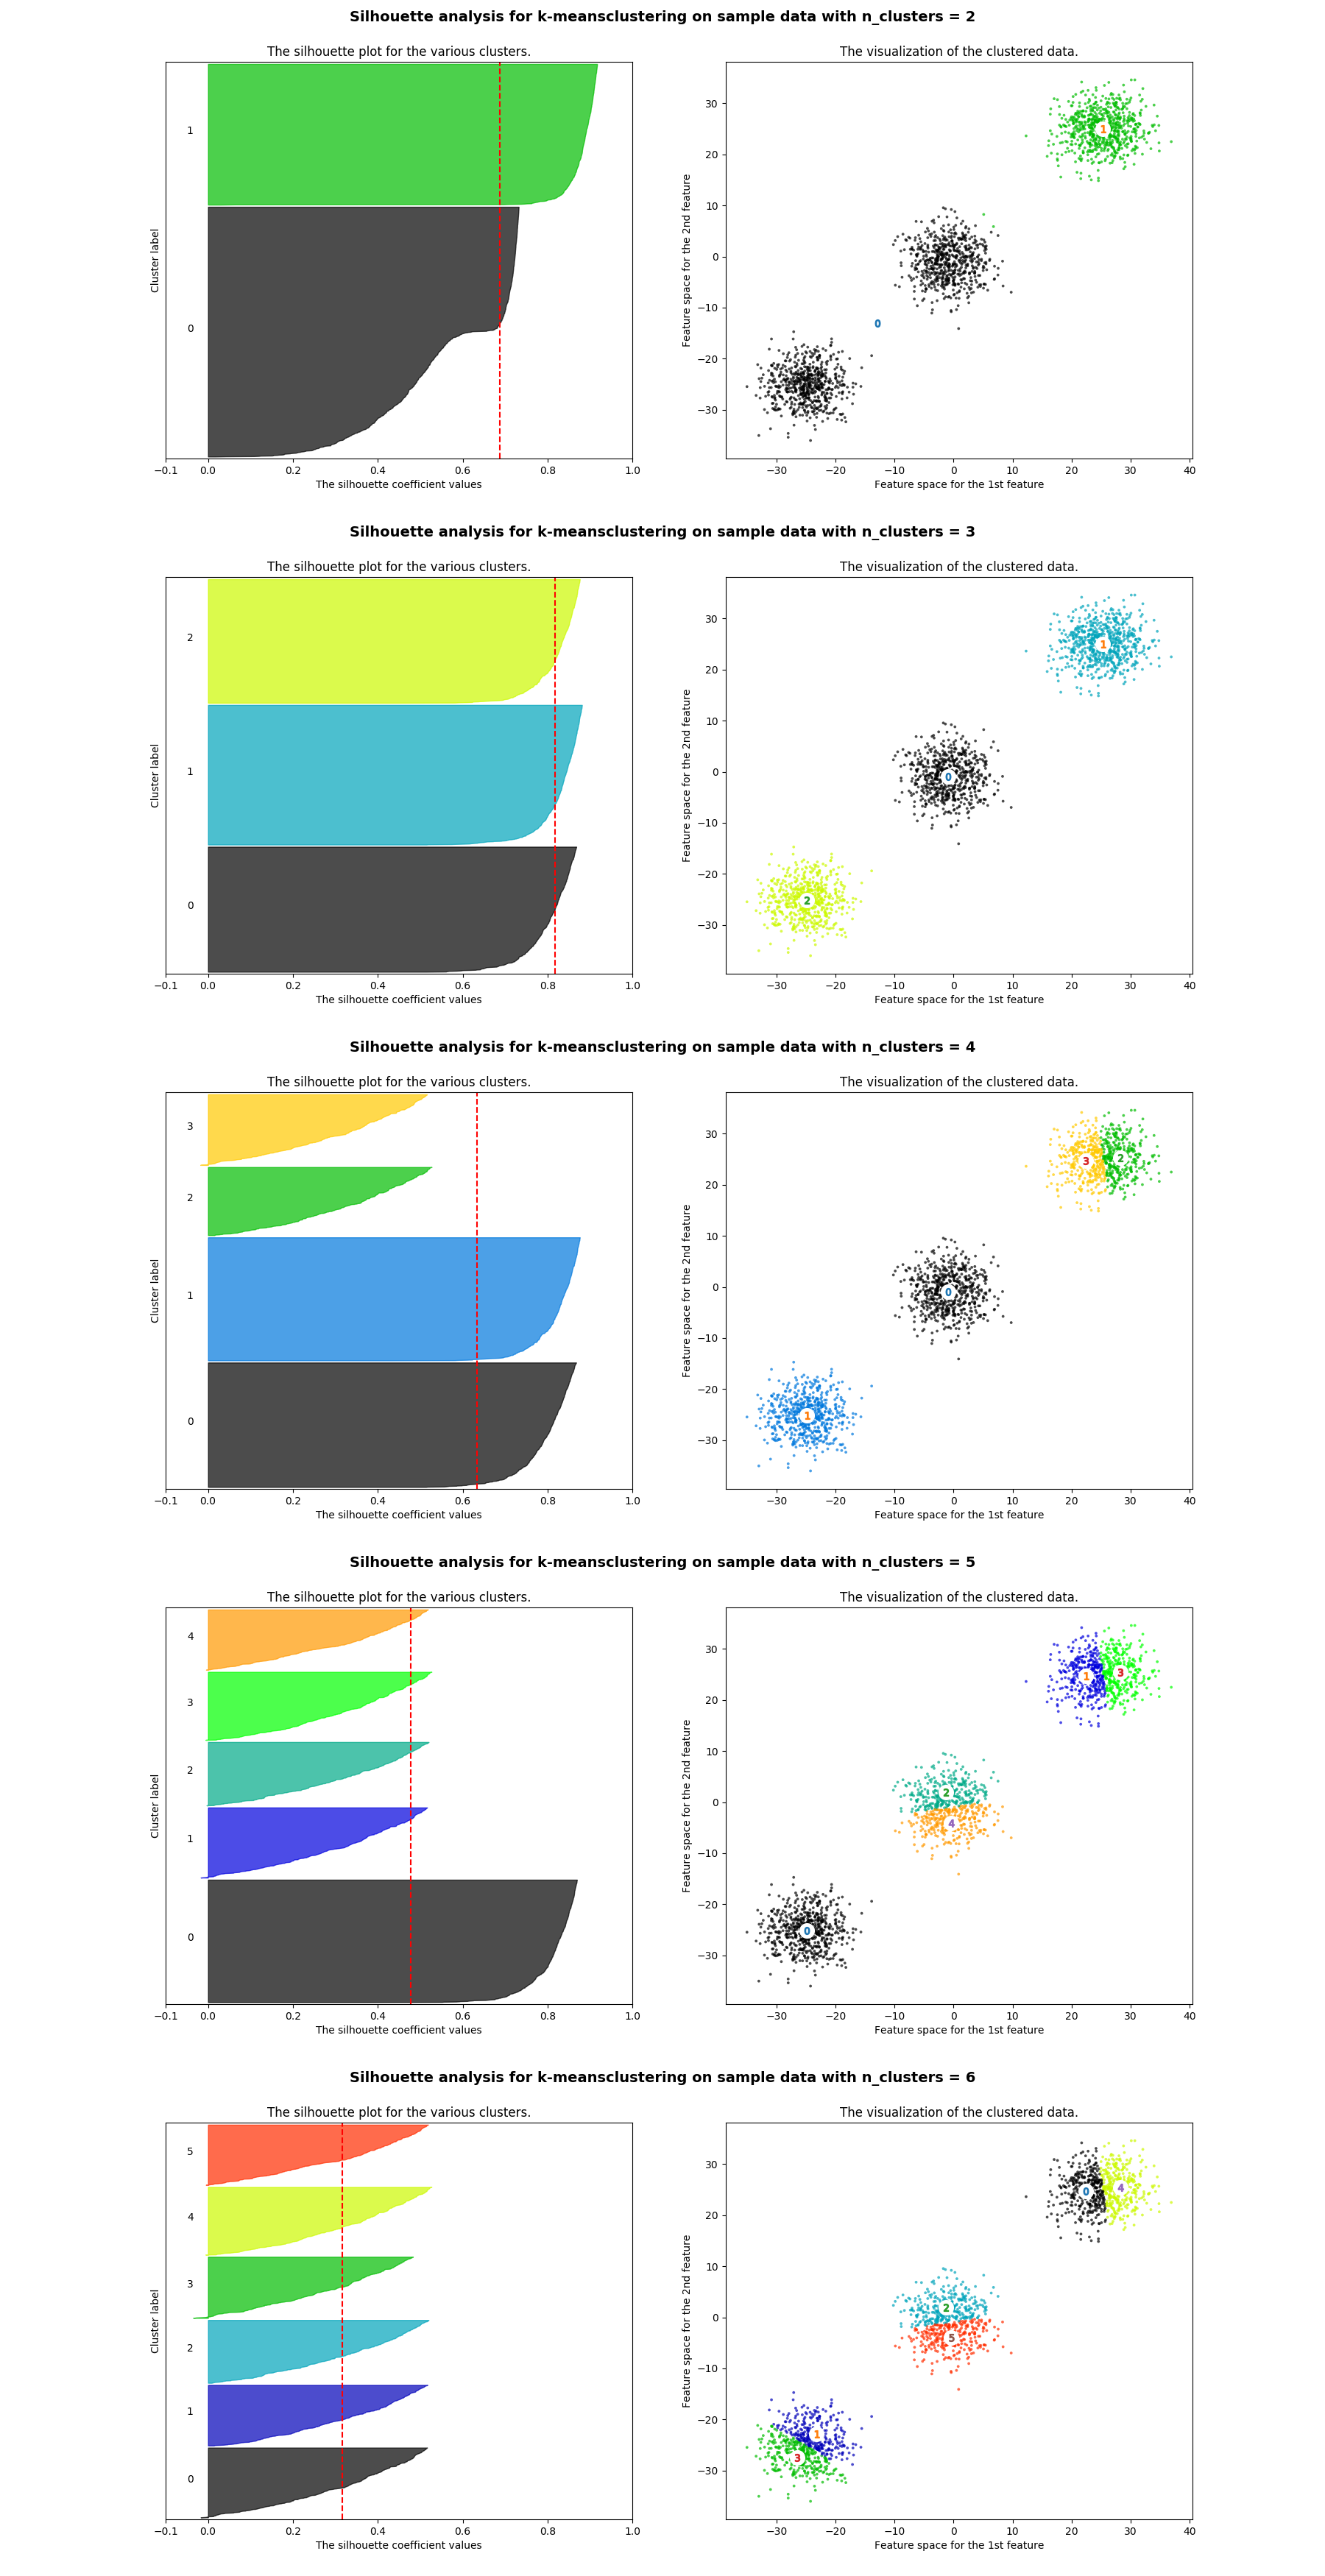
\includegraphics{../images/clustersScore.png}}
\end{center}
\begin{lstlisting} [language=Python]
"""
plotSilhouetteScore.py: Selecting the number of clusters with
                     silhouette analysis on k-means clustering.

Silhouette analysis can be used to study the separation distance between the
resulting clusters. The silhouette plot displays a measure of how close each
point in one cluster is to points in the neighboring clusters and thus provides
a way to assess parameters like number of clusters visually. This measure has a
range of [-1, 1].

Silhouette coefficients (as these values are referred to as) near +1 indicate
that the sample is far away from the neighboring clusters. A value of 0
indicates that the sample is on or very close to the decision boundary between
two neighboring clusters and negative values indicate that those samples might
have been assigned to the wrong cluster.

Source:
http://scikit-learn.org/stable/auto_examples/cluster/plot_kmeans_silhouette_analysis.html

"""

import argparse
from kmeans import KmeansRunner
import matplotlib.cm as cm
import matplotlib.pyplot as plt
import numpy as np
import os
import PIL
from sklearn.cluster import KMeans
from sklearn.metrics import silhouette_samples, silhouette_score

__author__ = "Scikit-Learn"


class SilhouetteScore():

    def calculateSilhouetteScore(self, dataFile):
        """Calculate the silhouette score for different numbers of clusters.

        :param self: An instance of the class SilhouetteScore.
        :param dataFile: An array with the input data points.
        :return: A list with the names of the image files created.
        """
        instanceKmeans = KmeansRunner()
        X = instanceKmeans.retrieveData(dataFile)
        if (X.shape[0] > 10000):
            size = round(X.shape[0] * 0.001)
            idx = np.random.randint(X.shape[0], size=size)
            subset = X[idx, :]
            X = subset
        range_n_clusters = [2, 3, 4, 5, 6]
        list_images = []

        for n_clusters in range_n_clusters:

            fig, (ax1, ax2) = plt.subplots(1, 2)
            fig.set_size_inches(18, 7)

            ax1.set_xlim([-0.1, 1])

            ax1.set_ylim([0, len(X) + (n_clusters + 1) * 10])

            clusterer = KMeans(n_clusters=n_clusters, random_state=10)
            cluster_labels = clusterer.fit_predict(np.array(X))

            silhouette_avg = silhouette_score(X, cluster_labels)
            print("For n_clusters =", n_clusters,
                  "The average silhouette_score is :", silhouette_avg)

            sample_silhouette_values = silhouette_samples(X, cluster_labels)

            y_lower = 10
            for i in range(n_clusters):

                ith_cluster_silhouette_values = \
                    sample_silhouette_values[cluster_labels == i]

                ith_cluster_silhouette_values.sort()

                size_cluster_i = ith_cluster_silhouette_values.shape[0]
                y_upper = y_lower + size_cluster_i

                color = cm.spectral(float(i) / n_clusters)
                ax1.fill_betweenx(np.arange(y_lower, y_upper),
                                  0, ith_cluster_silhouette_values,
                                  facecolor=color, edgecolor=color, alpha=0.7)

                ax1.text(-0.05, y_lower + 0.5 * size_cluster_i, str(i))

                y_lower = y_upper + 10

            ax1.set_title("The silhouette plot for the various clusters.")
            ax1.set_xlabel("The silhouette coefficient values")
            ax1.set_ylabel("Cluster label")

            ax1.axvline(x=silhouette_avg, color="red", linestyle="--")

            ax1.set_yticks([])
            ax1.set_xticks([-0.1, 0, 0.2, 0.4, 0.6, 0.8, 1])

            colors = cm.spectral(cluster_labels.astype(float) / n_clusters)
            ax2.scatter(X[:, 0], X[:, 1], marker=".", s=30, lw=0, alpha=0.7,
                        c=colors)

            centers = clusterer.cluster_centers_
            ax2.scatter(centers[:, 0], centers[:, 1],
                        marker="o", c="white", alpha=1, s=200)

            for i, c in enumerate(centers):
                ax2.scatter(c[0], c[1], marker="$%d$" % i, alpha=1, s=50)

            ax2.set_title("The visualization of the clustered data.")
            ax2.set_xlabel("Feature space for the 1st feature")
            ax2.set_ylabel("Feature space for the 2nd feature")

            plt.suptitle(("Silhouette analysis for k-means"
                          "clustering on sample data "
                          "with n_clusters = %d" % n_clusters),
                         fontsize=14, fontweight="bold")
            fig.savefig("cluster_" + str(n_clusters) + ".png")
            list_images.append("cluster_" + str(n_clusters) + ".png")
        return list_images

    def silhouetteScoretoPNG(self, list_images):
        """Save the results of the plots in asingle image file.

        :param self: An instance of the class SilhouetteScore.
        :param list_images: A list with the name of the image files created.
        """
        clusterImages = [PIL.Image.open(i) for i in list_images]
        minSize = sorted([(np.sum(i.size), i.size)
                          for i in clusterImages])[0][1]

        imagesCombination = np.vstack((np.asarray(i.resize(minSize))
                                       for i in clusterImages))
        imagesCombination = PIL.Image.fromarray(imagesCombination)
        directory = "../images"
        if not os.path.isdir(directory):
            os.makedirs(directory)
        imagesCombination.save("../images/clustersScore.png")
        for image in list_images:
            os.remove(image)
        print ("The silhouette score for the number of"
               " clusters ranging from 2 "
               "to 6 has been saved in the file clustersScore.png!")


if __name__ == "__main__":

    parser = argparse
    parser = argparse.ArgumentParser()
    parser.add_argument("dataFile", type=str,
                        help="File to retrieve the generated data points.")
    args = parser.parse_args()
    instanceSilhouetteScore = SilhouetteScore()
    images = instanceSilhouetteScore.calculateSilhouetteScore(args.dataFile)
    instanceSilhouetteScore.silhouetteScoretoPNG(images)

\end{lstlisting}

    

\section{k-means clustering
 algorithm}\label{k-means-clustering-algorithm}

\subsection{kmeans.py}\label{kmeans.py}

This python script calls the k-means algorithm implemented on hadoop.
However, before implementing k-means the initial centroids are computed
using the k-means++ algorithm proposed in 2007 by Arthur and
Vassilvitskii. 
\begin{algorithm}
	\caption{k-means++ algorithm}
							
	\begin{enumerate}
		\item Take one center $\displaystyle c_{1} $, chosen uniformly at random from $\displaystyle X $.
		\item Take a new center $\displaystyle c_{1} $, choosing  $\displaystyle {x\in X} $ with probability $\displaystyle \frac{D(x')^2}{\sum_{x\in X} {D(x')^2}} $.
		\item Repeat Step 2. until we have taken $\displaystyle k $ centers altogether.
		\item Proceed as with the standard k-means algorithm.
	\end{enumerate}
\end{algorithm}
\\\\
After determining the initial centroids, k-means algorithm is called in
order to detetermine the new centroids of the clusters and the results
are saved as an image file.

\begin{lstlisting}[language=Python]
"""kmeans.py: Run the k-means algorithm."""

import argparse
import matplotlib.pyplot as plt
import numpy as np
import pandas as pd
import os
import random
import re
import sys
sys.tracebacklimit = 0

__author__ = "Stratos Gounidellis, Lamprini Koutsokera"
__copyright__ = "Copyright 2017, BDSMasters"


class KmeansRunner():

    def retrieveData(self, file):
        """Retrieve the data points from the input file.

        :param self: An instance of the class KmeansRunner.
        :param file: A file with the input data.
        :return: An array with the input data points.
        """
        df_points = pd.read_csv(file, header=None, names=["x", "y"], sep=" ")
        if (len(df_points.index) < 1):
            raise Exception("The input file is empty!")
        data = [tuple(row) for row in df_points.values]
        points = np.array([data_point for data_point in data])
        return points

    def initialCentroids(self, file, nclusters):
        """Calculate the initial centroids to be used by the k-means
            clustering algorithm.

        :param self: An instance of the class KmeansRunner.
        :param file: A file with the input data.
        :param nclusters: The number of clusters.
        :return: A list with the initial centroids.
        """
        points = self.retrieveData(file)
        initial_centroids = [list(random.choice(points))]
        dist = []
        if nclusters < 2:
            raise Exception("Error the number of clusters should be" +
                            " greater than or equal to 2!")
        for i in range(2, nclusters + 1):
            dist.append([np.linalg.norm(np.array(point) -
                        initial_centroids[i - 2])**2 for point in points])
            min_dist = dist[0]
            if (len(dist) > 1):
                min_dist = np.minimum(
                    min_dist, (dist[index] for index in range(1, len(dist))))

            sumValues = sum(min_dist)
            probabilities = [float(value) / sumValues for value in min_dist]
            cumulative = np.cumsum(probabilities)

            random_index = random.random()
            index = np.where(cumulative >= random_index)[0][0]
            initial_centroids.append(list(points[index]))

        return initial_centroids

    def retrieveCentroids(self, file):
        """Retrieve the centroids coordinated from the centroids file.

        :param self: An instance of the class KmeansRunner.
        :param file: A file with the centroids.
        :return: A list with the centroids.
        """
        with open(file, "r") as inputFile:
            output_data = inputFile.readlines()

        centroids = []
        for point in output_data:
            p = re.search("\[(.*?)\]", point).group()
            p = p.replace("[", "").replace("]", "")
            p.strip()
            axisx, axisy = p.split(",")
            axisx = float(axisx)
            axisy = float(axisy)
            point_list = [axisx, axisy]
            centroids.append(point_list)
        return centroids

    def retrieveLabels(self, dataFile, centroidsFile):
        """Retrieve the labels of the imput data points.

        :param self: An instance of the class KmeansRunner.
        :param dataFile: A file with the input data points.
        :param centroidsFile: A file with the centroids.
        :return: A list with the labels.
        """
        data_points = self.retrieveData(dataFile)
        centroids = self.retrieveCentroids(centroidsFile)
        labels = []
        for data_point in data_points:
            distances = [np.linalg.norm(data_point - centroid)
                         for centroid in centroids]
            cluster = np.argmin(distances)
            labels.append(int(cluster))
        return labels

    def writeCentroids(self, centroids, file):
        """Write centroids to a file.

        :param self: An instance of the class KmeansRunner.
        :param centroids: A list with the centroids.
        :param file: A file to write the centroids.
        """
        f = open(CENTROIDS_FILE, "w+")
        for item in centroids:
            f.write("%s\n" % str(item))
        f.close()

    def plotClusters(self, data_points, centroids, labels):
        """Plot the clusters with the centroids and save the plot as an image.

        :param self: An instance of the class KmeansRunner.
        :param data_points: An array with the input data points.
        :param centroids: A list with the centroids.
        :param labels: The labels of the input data points.
        """
        plt.scatter(data_points[:, 0], data_points[:, 1], c=labels)
        for i in range(len(centroids)):
            label = "Centroid " + str(i)
            colors = ["red", "green", "blue"]
            plt.scatter(centroids[i][0], centroids[i][1], s=50,
                        c=colors[i], label=label)
        plt.legend(loc="best", fancybox=True)
        fig = plt.gcf()
        plt.show()
        directory = "../images"
        if not os.path.isdir(directory):
            os.makedirs(directory)
        fig.savefig("../images/clusters.png")


CENTROIDS_FILE = "centroids.txt"
OUTPUT_FILE = "output.txt"

if __name__ == "__main__":

    parser = argparse
    parser = argparse.ArgumentParser(description="k-means algorithm"
                                     " implementation on Hadoop",
                                     epilog="Go ahead and try it!")
    parser.add_argument("inputFile", type=str,
                        help="Input data points for the clustering algorithm.")
    parser.add_argument("centroids", type=int,
                        help="Number of clusters.")
    args = parser.parse_args()

    data = args.inputFile
    k = args.centroids
    instanceKmeans = KmeansRunner()
    centroids = instanceKmeans.initialCentroids(data, int(k))
    instanceKmeans.writeCentroids(centroids, CENTROIDS_FILE)

    outputFile = open(OUTPUT_FILE, "w+")
    outputFile.close()

    i = 1
    while True:
        print "k-means iteration #%i" % i

        command = "python kmeansAlgorithm.py < " \
                  + data + " --k=" \
                  + str(k) + " --centroids=" \
                  + CENTROIDS_FILE + " > " + OUTPUT_FILE \
                  + " -r hadoop"
        os.popen(command)

        new_centroids = instanceKmeans.retrieveCentroids(OUTPUT_FILE)

        if sorted(centroids) != sorted(new_centroids):
            centroids = new_centroids
            instanceKmeans.writeCentroids(centroids, CENTROIDS_FILE)
        else:
            break
        i += 1

    os.remove(OUTPUT_FILE)
    labels = instanceKmeans.retrieveLabels(data, CENTROIDS_FILE)
    labelsFile = open("labels.txt", "w+")
    for label in labels:
        labelsFile.write("%s\n" % str(label))
    labelsFile.close()
    data_points = instanceKmeans.retrieveData(data)
    instanceKmeans.plotClusters(data_points, centroids, labels)

\end{lstlisting}

\subsection{kmeansAlgorithm.py}\label{kmeansAlgorithm.py}
In order to implement k-means algorithm on hadoop mrjob is used. Mrjob is
a python package, which allows to write multi-step MapReduce jobs in
pure Python and run them on a hadoop cluster. In our case mrjob run on a
single-node cluster. (The script can also be run locally by commenting the argument ``-r hadoop''.) 

\begin{algorithm}
	\caption{k-means algorithm}
							
	\begin{enumerate}
		\item Define the number of clusters, k.
		\item Select k data points as initial centroids. 
		\item Assign each data object to the closest cluster centroid.
		\item Recalculate the clusters’ centroids.
		\item  If the centroids remain unchanged the algorithm terminates. Otherwise, the steps are repeated from Step 2.
	\end{enumerate}
\end{algorithm}

\begin{algorithm}
	\caption{k-means algorithm - MapReduce}
							
	\begin{enumerate}
		\item The mapper function returns each data point and the cluster, to which it belongs.
		\item The combiner function returns partial sums of batches of data points belonging to the same cluster. 
		\item The reducer returns the new centroids of each cluster.
		\item If the centroids remain unchanged the algorithm terminates. Otherwise, the steps are repeated from the beginning.
	\end{enumerate}
							
\end{algorithm}


\begin{center}
	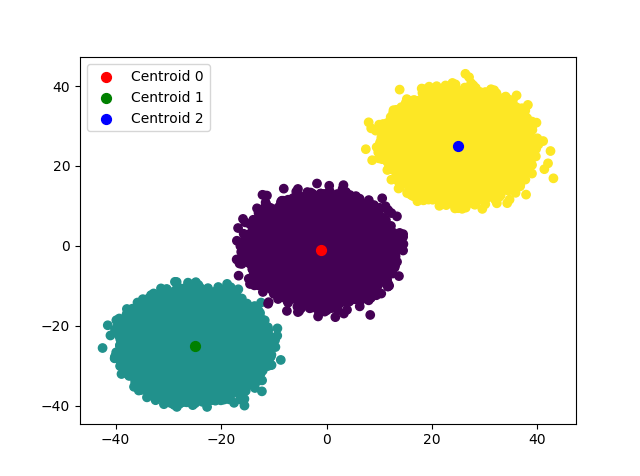
\includegraphics{../images/clusters.png}\\
\end{center}
\begin{lstlisting}[language=Python]
"""kmeansAlgorithm.py: Implement the k-means clustering
    algorithm on the input data."""

from mrjob.job import MRJob
from mrjob.job import MRStep
import numpy as np
import re

__author__ = "Stratos Gounidellis, Lamprini Koutsokera"
__copyright__ = "Copyright 2017, BDSMasters"


class KmeansAlgorithm(MRJob):
    def configure_options(self):
        """Set the arguments for the class KmeansAlgorithm.

        :param self: A instance of the class KmeansAlgorithm.
        """
        super(KmeansAlgorithm, self).configure_options()
        self.add_passthrough_option(
            "--k", type="int", help="Number of clusters.")
        self.add_file_option("--centroids")

    def retrieveCentroids(self, file):
        """Retrieve the centroids coordinated from the centroids file.

        :param self: An instance of the class KmeansAlgorithm.
        :param file: A file with the centroids.
        :return: A list with the centroids.
        """
        with open(file, "r") as inputFile:
            output_data = inputFile.readlines()

        centroids = []
        for point in output_data:
            p = re.search("\[(.*?)\]", point).group()
            p = p.replace("[", "").replace("]", "")
            p.strip()
            axisx, axisy = p.split(",")
            axisx = float(axisx)
            axisy = float(axisy)
            point_list = [axisx, axisy]
            centroids.append(point_list)
        return centroids

    def assignPointtoCluster(self, _, line):
        """Assign each point to its closest cluster - Mapper Function.

        :param self: An instance of the class KmeansAlgorithm.
        :param line: A line from the input data, with data points in
            the form [axisx axisy]
        :yield: The identifier of a cluster and a point belonging to it.
        """
        axisx, axisy = line.split()
        data_point = np.array([float(axisx), float(axisy)])
        centroids = self.retrieveCentroids(self.options.centroids)
        distances = [np.linalg.norm(data_point - centroid)
                     for centroid in centroids]
        cluster = np.argmin(distances)
        yield int(cluster), data_point.tolist()

    def calculatePartialSum(self, cluster, data_points):
        """Calculate the partial sum of the data points belonging to
            each cluster - Combiner Function.

        :param self: An instance of the class KmeansAlgorithm.
        :param cluster: An identifier for each cluster.
        :param data_points: A list of points belonging to each cluster.
        :yield: The identifier of a cluster, the partial sum of its
            data points and their number.
        """
        sum_points = np.array(data_points.next())
        counter = 1
        for data_point in data_points:
            sum_points += data_point
            counter += 1
        yield cluster, (sum_points.tolist(), counter)

    def calculateNewCentroids(self, cluster, partial_sums):
        """Calculate the new centroids of the clusters - Reduce Function.

        :param self: An instance of the class KmeansAlgorithm.
        :param cluster: An identifier for each cluster.
        :param partial_sums: A list with the partial sum of the
            data points of a cluster and their number.
        :yield: The identifier of a cluster and its new centroid.
        """
        total_sum, total_counter = partial_sums.next()
        total_sum = np.array(total_sum)
        for partial_sum, counter in partial_sums:
            total_sum += partial_sum
            total_counter += counter
        yield cluster, (total_sum / total_counter).tolist()

    def steps(self):
        """Set the steps of the MRJob.

        :param self: An instance of the class KmeansAlgorithm.

        :return: a list of steps constructed with MRStep().
        """
        return [MRStep(mapper=self.assignPointtoCluster,
                combiner=self.calculatePartialSum,
                reducer=self.calculateNewCentroids)]


if __name__ == "__main__":
    KmeansAlgorithm.run()

\end{lstlisting}


\section{Testing Functionality}\label{number-of-clusters}
\subsection{test.py}\label{test.py}
\begin{lstlisting} [language=Python]
import unittest
from createDataPoints import DataGenerator
from kmeans import KmeansRunner

__author__ = "Stratos Gounidellis, Lamprini Koutsokera"
__copyright__ = "Copyright 2017, BDSMasters"


class TestStringMethods(unittest.TestCase):

    def test_dataPoints(self):
        instanceData = DataGenerator()
        fname = "test.txt"
        instanceData.generateData(100, fname)
        with open(fname) as f:
            for i, l in enumerate(f):
                pass
        i + 1
        self.assertEqual(100, i+1)

    def test_exceptionClustersNumber(self):
        fname = "test.txt"
        instanceKmeans = KmeansRunner()
        with self.assertRaises(Exception) as context:
            instanceKmeans.initialCentroids(fname, 1)
        self.assertIn("Error the number of clusters should be greater" +
                      "than or equal to 2!", "".join(context.exception))

    def test_fileLength(self):
        fname = "test.txt"
        instanceKmeans = KmeansRunner()
        testFile = open(fname, "w+")
        testFile.close()
        with self.assertRaises(Exception) as context:
            instanceKmeans.retrieveData(fname)
        self.assertIn("The input file is empty!", "".join(context.exception))


if __name__ == "__main__":
    unittest.main()

\end{lstlisting}

\phantomsection 
\addcontentsline{toc}{section}{References} 

\begin{thebibliography}{9}
	\bibitem{hadoopconfiguration} 
	Michael G. Noll.
	\textit{Running Hadoop On Ubuntu Linux (Single-Node Cluster)}. 
	\url {http://www.michael-noll.com/tutorials/running-hadoop-on-ubuntu-linux-single-node-cluster/}
	[\textit{Accessed 29 Mar. 2017}]. 
							
	\bibitem{mrjobconfiguration} 
	Stackoverflow.com.
	\textit{Error launching job using mrjob on Hadoop}. 
	\url {http://stackoverflow.com/questions/25358793/error-launching-job-using-mrjob-on-hadoop}
	[\textit{Accessed 29 Mar. 2017}].
							
	\bibitem{k-means++} 
	David Arthur, and Sergei Vassilvitskii (2007). 
	\textit{k-means++: the advantages of careful seeding }
	Proceedings of the eighteenth annual ACM-SIAM Symposium on Discrete Algorithms, New Orleans, LA, January 7-9, 2007. 1st ed. New York: ACM, pp.1027–1035.
							
	\bibitem{kmeans} 
	Nlp.stanford.edu.
	\textit{Kmeans}. 
	\url {http://nlp.stanford.edu/IR-book/html/htmledition/k-means-1.html}
	[\textit{Accessed 15 Mar. 2017}].
							
	\bibitem{kmeans_cluster} 
	Home.deib.polimi.it.
	\textit{Clustering - K-means}. 
	\url {http://home.deib.polimi.it/matteucc/Clustering/tutorial\_html/kmeans.html}
	[\textit{Accessed 8 Mar. 2017}].
							
	\bibitem{kmeans_mapreduce} 
	Kyuseok Shim.
	\textit{MapReduce Algorithms for Big Data Analysis}. 
	VLDB Conference, 2012.
							
\end{thebibliography}
\end{document}